\chapter{Mathe - Klasse 1}
\section{Übungen 2}
Rechne aus: \\ \\
\begin{tabular}{p{3cm}p{3cm}p{3cm}p{3cm}p{3cm}}
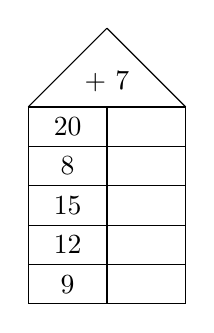
\begin{tikzpicture}
% Figur-Körper
\draw ( 0, 0 ) -- ( 1,  1 );
\draw ( 2, 0 ) -- ( 0,  0 );
\draw ( 2, 0 ) -- ( 1,  1 );
\draw ( 2, 0 ) -- ( 2, -2.5 );
\draw ( 0, 0 ) -- ( 0, -2.5 );

\draw ( 0, -0.5) -- ( 2, -0.5 );
\draw ( 0, -1.0) -- ( 2, -1.0 );
\draw ( 0, -1.5) -- ( 2, -1.5 );
\draw ( 0, -2.0) -- ( 2, -2.0 );
\draw ( 0, -2.5) -- ( 2, -2.5 );

% Teiler (r/l)
\draw ( 1, -2.5) -- ( 1, 0 );
\draw ( 1, 0.32) node { + 7 };

\draw ( 0.5, -0.25 ) node { 20 };
\draw ( 0.5, -0.75 ) node {  8 };
\draw ( 0.5, -1.25 ) node { 15 };
\draw ( 0.5, -1.75 ) node { 12 };
\draw ( 0.5, -2.25 ) node {  9 };
\end{tikzpicture}

&

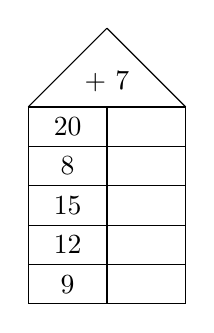
\begin{tikzpicture}
\draw ( 0, 0 ) -- ( 1,  1 );
\draw ( 2, 0 ) -- ( 0,  0 );
\draw ( 2, 0 ) -- ( 1,  1 );
\draw ( 2, 0 ) -- ( 2, -2.5 );
\draw ( 0, 0 ) -- ( 0, -2.5 );

\draw ( 0, -0.5) -- ( 2, -0.5 );
\draw ( 0, -1.0) -- ( 2, -1.0 );
\draw ( 0, -1.5) -- ( 2, -1.5 );
\draw ( 0, -2.0) -- ( 2, -2.0 );
\draw ( 0, -2.5) -- ( 2, -2.5 );

% Teiler (r/l)
\draw ( 1, -2.5) -- ( 1, 0 );
\draw ( 1, 0.32) node { + 7 };

\draw ( 0.5, -0.25 ) node { 20 };
\draw ( 0.5, -0.75 ) node {  8 };
\draw ( 0.5, -1.25 ) node { 15 };
\draw ( 0.5, -1.75 ) node { 12 };
\draw ( 0.5, -2.25 ) node {  9 };

\end{tikzpicture}

&

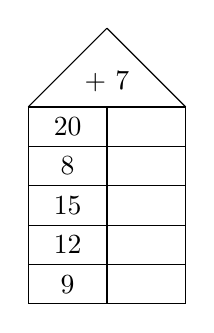
\begin{tikzpicture}
\draw ( 0, 0 ) -- ( 1,  1 );
\draw ( 2, 0 ) -- ( 0,  0 );
\draw ( 2, 0 ) -- ( 1,  1 );
\draw ( 2, 0 ) -- ( 2, -2.5 );
\draw ( 0, 0 ) -- ( 0, -2.5 );

\draw ( 0, -0.5) -- ( 2, -0.5 );
\draw ( 0, -1.0) -- ( 2, -1.0 );
\draw ( 0, -1.5) -- ( 2, -1.5 );
\draw ( 0, -2.0) -- ( 2, -2.0 );
\draw ( 0, -2.5) -- ( 2, -2.5 );

% Teiler (r/l)
\draw ( 1, -2.5) -- ( 1, 0 );
\draw ( 1, 0.32) node { + 7 };

\draw ( 0.5, -0.25 ) node { 20 };
\draw ( 0.5, -0.75 ) node {  8 };
\draw ( 0.5, -1.25 ) node { 15 };
\draw ( 0.5, -1.75 ) node { 12 };
\draw ( 0.5, -2.25 ) node {  9 };

\end{tikzpicture}

&

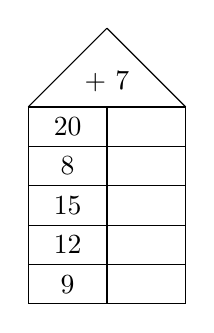
\begin{tikzpicture}
\draw ( 0, 0 ) -- ( 1,  1 );
\draw ( 2, 0 ) -- ( 0,  0 );
\draw ( 2, 0 ) -- ( 1,  1 );
\draw ( 2, 0 ) -- ( 2, -2.5 );
\draw ( 0, 0 ) -- ( 0, -2.5 );

\draw ( 0, -0.5) -- ( 2, -0.5 );
\draw ( 0, -1.0) -- ( 2, -1.0 );
\draw ( 0, -1.5) -- ( 2, -1.5 );
\draw ( 0, -2.0) -- ( 2, -2.0 );
\draw ( 0, -2.5) -- ( 2, -2.5 );

% Teiler (r/l)
\draw ( 1, -2.5) -- ( 1, 0 );
\draw ( 1, 0.32) node { + 7 };

\draw ( 0.5, -0.25 ) node { 20 };
\draw ( 0.5, -0.75 ) node {  8 };
\draw ( 0.5, -1.25 ) node { 15 };
\draw ( 0.5, -1.75 ) node { 12 };
\draw ( 0.5, -2.25 ) node {  9 };

\end{tikzpicture}

&

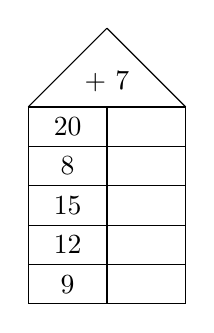
\begin{tikzpicture}
\draw ( 0, 0 ) -- ( 1,  1 );
\draw ( 2, 0 ) -- ( 0,  0 );
\draw ( 2, 0 ) -- ( 1,  1 );
\draw ( 2, 0 ) -- ( 2, -2.5 );
\draw ( 0, 0 ) -- ( 0, -2.5 );

\draw ( 0, -0.5) -- ( 2, -0.5 );
\draw ( 0, -1.0) -- ( 2, -1.0 );
\draw ( 0, -1.5) -- ( 2, -1.5 );
\draw ( 0, -2.0) -- ( 2, -2.0 );
\draw ( 0, -2.5) -- ( 2, -2.5 );

% Teiler (r/l)
\draw ( 1, -2.5) -- ( 1, 0 );
\draw ( 1, 0.32) node { + 7 };

\draw ( 0.5, -0.25 ) node { 20 };
\draw ( 0.5, -0.75 ) node {  8 };
\draw ( 0.5, -1.25 ) node { 15 };
\draw ( 0.5, -1.75 ) node { 12 };
\draw ( 0.5, -2.25 ) node {  9 };

\end{tikzpicture}
\end{tabular}

\vspace{2cm}
%--------------------------

\begin{tabular}{p{3cm}p{3cm}p{3cm}p{3cm}p{3cm}}
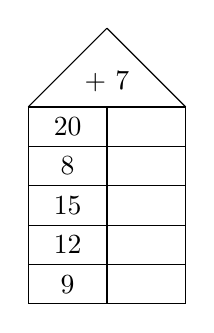
\begin{tikzpicture}
% Figur-Körper
\draw ( 0, 0 ) -- ( 1,  1 );
\draw ( 2, 0 ) -- ( 0,  0 );
\draw ( 2, 0 ) -- ( 1,  1 );
\draw ( 2, 0 ) -- ( 2, -2.5 );
\draw ( 0, 0 ) -- ( 0, -2.5 );

\draw ( 0, -0.5) -- ( 2, -0.5 );
\draw ( 0, -1.0) -- ( 2, -1.0 );
\draw ( 0, -1.5) -- ( 2, -1.5 );
\draw ( 0, -2.0) -- ( 2, -2.0 );
\draw ( 0, -2.5) -- ( 2, -2.5 );

% Teiler (r/l)
\draw ( 1, -2.5) -- ( 1, 0 );
\draw ( 1, 0.32) node { + 7 };

\draw ( 0.5, -0.25 ) node { 20 };
\draw ( 0.5, -0.75 ) node {  8 };
\draw ( 0.5, -1.25 ) node { 15 };
\draw ( 0.5, -1.75 ) node { 12 };
\draw ( 0.5, -2.25 ) node {  9 };
\end{tikzpicture}

&

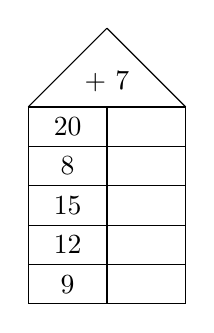
\begin{tikzpicture}
\draw ( 0, 0 ) -- ( 1,  1 );
\draw ( 2, 0 ) -- ( 0,  0 );
\draw ( 2, 0 ) -- ( 1,  1 );
\draw ( 2, 0 ) -- ( 2, -2.5 );
\draw ( 0, 0 ) -- ( 0, -2.5 );

\draw ( 0, -0.5) -- ( 2, -0.5 );
\draw ( 0, -1.0) -- ( 2, -1.0 );
\draw ( 0, -1.5) -- ( 2, -1.5 );
\draw ( 0, -2.0) -- ( 2, -2.0 );
\draw ( 0, -2.5) -- ( 2, -2.5 );

% Teiler (r/l)
\draw ( 1, -2.5) -- ( 1, 0 );
\draw ( 1, 0.32) node { + 7 };

\draw ( 0.5, -0.25 ) node { 20 };
\draw ( 0.5, -0.75 ) node {  8 };
\draw ( 0.5, -1.25 ) node { 15 };
\draw ( 0.5, -1.75 ) node { 12 };
\draw ( 0.5, -2.25 ) node {  9 };

\end{tikzpicture}

&

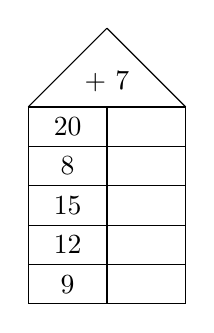
\begin{tikzpicture}
\draw ( 0, 0 ) -- ( 1,  1 );
\draw ( 2, 0 ) -- ( 0,  0 );
\draw ( 2, 0 ) -- ( 1,  1 );
\draw ( 2, 0 ) -- ( 2, -2.5 );
\draw ( 0, 0 ) -- ( 0, -2.5 );

\draw ( 0, -0.5) -- ( 2, -0.5 );
\draw ( 0, -1.0) -- ( 2, -1.0 );
\draw ( 0, -1.5) -- ( 2, -1.5 );
\draw ( 0, -2.0) -- ( 2, -2.0 );
\draw ( 0, -2.5) -- ( 2, -2.5 );

% Teiler (r/l)
\draw ( 1, -2.5) -- ( 1, 0 );
\draw ( 1, 0.32) node { + 7 };

\draw ( 0.5, -0.25 ) node { 20 };
\draw ( 0.5, -0.75 ) node {  8 };
\draw ( 0.5, -1.25 ) node { 15 };
\draw ( 0.5, -1.75 ) node { 12 };
\draw ( 0.5, -2.25 ) node {  9 };

\end{tikzpicture}

&

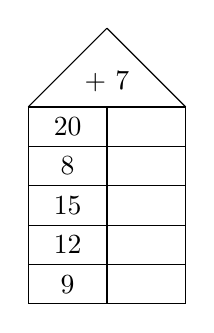
\begin{tikzpicture}
\draw ( 0, 0 ) -- ( 1,  1 );
\draw ( 2, 0 ) -- ( 0,  0 );
\draw ( 2, 0 ) -- ( 1,  1 );
\draw ( 2, 0 ) -- ( 2, -2.5 );
\draw ( 0, 0 ) -- ( 0, -2.5 );

\draw ( 0, -0.5) -- ( 2, -0.5 );
\draw ( 0, -1.0) -- ( 2, -1.0 );
\draw ( 0, -1.5) -- ( 2, -1.5 );
\draw ( 0, -2.0) -- ( 2, -2.0 );
\draw ( 0, -2.5) -- ( 2, -2.5 );

% Teiler (r/l)
\draw ( 1, -2.5) -- ( 1, 0 );
\draw ( 1, 0.32) node { + 7 };

\draw ( 0.5, -0.25 ) node { 20 };
\draw ( 0.5, -0.75 ) node {  8 };
\draw ( 0.5, -1.25 ) node { 15 };
\draw ( 0.5, -1.75 ) node { 12 };
\draw ( 0.5, -2.25 ) node {  9 };

\end{tikzpicture}

&

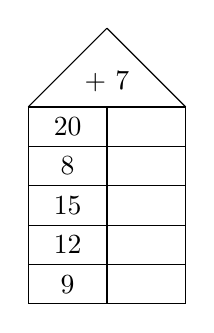
\begin{tikzpicture}
\draw ( 0, 0 ) -- ( 1,  1 );
\draw ( 2, 0 ) -- ( 0,  0 );
\draw ( 2, 0 ) -- ( 1,  1 );
\draw ( 2, 0 ) -- ( 2, -2.5 );
\draw ( 0, 0 ) -- ( 0, -2.5 );

\draw ( 0, -0.5) -- ( 2, -0.5 );
\draw ( 0, -1.0) -- ( 2, -1.0 );
\draw ( 0, -1.5) -- ( 2, -1.5 );
\draw ( 0, -2.0) -- ( 2, -2.0 );
\draw ( 0, -2.5) -- ( 2, -2.5 );

% Teiler (r/l)
\draw ( 1, -2.5) -- ( 1, 0 );
\draw ( 1, 0.32) node { + 7 };

\draw ( 0.5, -0.25 ) node { 20 };
\draw ( 0.5, -0.75 ) node {  8 };
\draw ( 0.5, -1.25 ) node { 15 };
\draw ( 0.5, -1.75 ) node { 12 };
\draw ( 0.5, -2.25 ) node {  9 };

\end{tikzpicture}
\end{tabular}

\vspace{2cm}
%--------------------------

\begin{tabular}{p{3cm}p{3cm}p{3cm}p{3cm}p{3cm}}
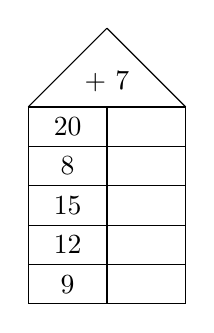
\begin{tikzpicture}
% Figur-Körper
\draw ( 0, 0 ) -- ( 1,  1 );
\draw ( 2, 0 ) -- ( 0,  0 );
\draw ( 2, 0 ) -- ( 1,  1 );
\draw ( 2, 0 ) -- ( 2, -2.5 );
\draw ( 0, 0 ) -- ( 0, -2.5 );

\draw ( 0, -0.5) -- ( 2, -0.5 );
\draw ( 0, -1.0) -- ( 2, -1.0 );
\draw ( 0, -1.5) -- ( 2, -1.5 );
\draw ( 0, -2.0) -- ( 2, -2.0 );
\draw ( 0, -2.5) -- ( 2, -2.5 );

% Teiler (r/l)
\draw ( 1, -2.5) -- ( 1, 0 );
\draw ( 1, 0.32) node { + 7 };

\draw ( 0.5, -0.25 ) node { 20 };
\draw ( 0.5, -0.75 ) node {  8 };
\draw ( 0.5, -1.25 ) node { 15 };
\draw ( 0.5, -1.75 ) node { 12 };
\draw ( 0.5, -2.25 ) node {  9 };
\end{tikzpicture}

&

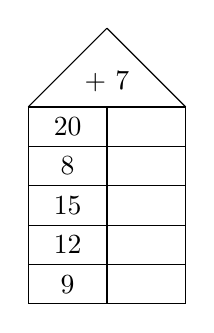
\begin{tikzpicture}
\draw ( 0, 0 ) -- ( 1,  1 );
\draw ( 2, 0 ) -- ( 0,  0 );
\draw ( 2, 0 ) -- ( 1,  1 );
\draw ( 2, 0 ) -- ( 2, -2.5 );
\draw ( 0, 0 ) -- ( 0, -2.5 );

\draw ( 0, -0.5) -- ( 2, -0.5 );
\draw ( 0, -1.0) -- ( 2, -1.0 );
\draw ( 0, -1.5) -- ( 2, -1.5 );
\draw ( 0, -2.0) -- ( 2, -2.0 );
\draw ( 0, -2.5) -- ( 2, -2.5 );

% Teiler (r/l)
\draw ( 1, -2.5) -- ( 1, 0 );
\draw ( 1, 0.32) node { + 7 };

\draw ( 0.5, -0.25 ) node { 20 };
\draw ( 0.5, -0.75 ) node {  8 };
\draw ( 0.5, -1.25 ) node { 15 };
\draw ( 0.5, -1.75 ) node { 12 };
\draw ( 0.5, -2.25 ) node {  9 };

\end{tikzpicture}

&

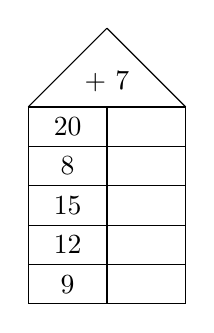
\begin{tikzpicture}
\draw ( 0, 0 ) -- ( 1,  1 );
\draw ( 2, 0 ) -- ( 0,  0 );
\draw ( 2, 0 ) -- ( 1,  1 );
\draw ( 2, 0 ) -- ( 2, -2.5 );
\draw ( 0, 0 ) -- ( 0, -2.5 );

\draw ( 0, -0.5) -- ( 2, -0.5 );
\draw ( 0, -1.0) -- ( 2, -1.0 );
\draw ( 0, -1.5) -- ( 2, -1.5 );
\draw ( 0, -2.0) -- ( 2, -2.0 );
\draw ( 0, -2.5) -- ( 2, -2.5 );

% Teiler (r/l)
\draw ( 1, -2.5) -- ( 1, 0 );
\draw ( 1, 0.32) node { + 7 };

\draw ( 0.5, -0.25 ) node { 20 };
\draw ( 0.5, -0.75 ) node {  8 };
\draw ( 0.5, -1.25 ) node { 15 };
\draw ( 0.5, -1.75 ) node { 12 };
\draw ( 0.5, -2.25 ) node {  9 };

\end{tikzpicture}

&

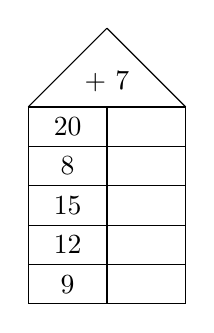
\begin{tikzpicture}
\draw ( 0, 0 ) -- ( 1,  1 );
\draw ( 2, 0 ) -- ( 0,  0 );
\draw ( 2, 0 ) -- ( 1,  1 );
\draw ( 2, 0 ) -- ( 2, -2.5 );
\draw ( 0, 0 ) -- ( 0, -2.5 );

\draw ( 0, -0.5) -- ( 2, -0.5 );
\draw ( 0, -1.0) -- ( 2, -1.0 );
\draw ( 0, -1.5) -- ( 2, -1.5 );
\draw ( 0, -2.0) -- ( 2, -2.0 );
\draw ( 0, -2.5) -- ( 2, -2.5 );

% Teiler (r/l)
\draw ( 1, -2.5) -- ( 1, 0 );
\draw ( 1, 0.32) node { + 7 };

\draw ( 0.5, -0.25 ) node { 20 };
\draw ( 0.5, -0.75 ) node {  8 };
\draw ( 0.5, -1.25 ) node { 15 };
\draw ( 0.5, -1.75 ) node { 12 };
\draw ( 0.5, -2.25 ) node {  9 };

\end{tikzpicture}

&

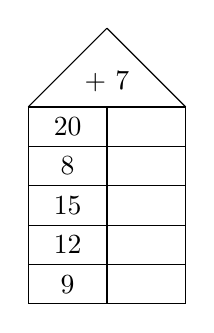
\begin{tikzpicture}
\draw ( 0, 0 ) -- ( 1,  1 );
\draw ( 2, 0 ) -- ( 0,  0 );
\draw ( 2, 0 ) -- ( 1,  1 );
\draw ( 2, 0 ) -- ( 2, -2.5 );
\draw ( 0, 0 ) -- ( 0, -2.5 );

\draw ( 0, -0.5) -- ( 2, -0.5 );
\draw ( 0, -1.0) -- ( 2, -1.0 );
\draw ( 0, -1.5) -- ( 2, -1.5 );
\draw ( 0, -2.0) -- ( 2, -2.0 );
\draw ( 0, -2.5) -- ( 2, -2.5 );

% Teiler (r/l)
\draw ( 1, -2.5) -- ( 1, 0 );
\draw ( 1, 0.32) node { + 7 };

\draw ( 0.5, -0.25 ) node { 20 };
\draw ( 0.5, -0.75 ) node {  8 };
\draw ( 0.5, -1.25 ) node { 15 };
\draw ( 0.5, -1.75 ) node { 12 };
\draw ( 0.5, -2.25 ) node {  9 };

\end{tikzpicture}
\end{tabular}
